%%
%% This is file `mcmthesis-demo.tex',
%% generated with the docstrip utility.
%%
%% The original source files were:
%%
%% mcmthesis.dtx  (with options: `demo')
%%
%% -----------------------------------
%%
%% This is a generated file.
%%
%% Copyright (C)
%%     2010 -- 2015 by Zhaoli Wang
%%     2014 -- 2016 by Liam Huang
%%     2016 -- 2018 by Xuehan Sun
%%
%% This work may be distributed and/or modified under the
%% conditions of the LaTeX Project Public License, either version 1.3
%% of this license or (at your option) any later version.
%%
%% This work has the LPPL maintenance status `maintained'.
%%
%% The Current Maintainer of this work is Xuehan Sun.
%%
\documentclass{mcmthesis}
\mcmsetup{CTeX = false,   % 使用 CTeX 套装时,设置为 true
        tcn = 011, problem = B,
        sheet = true, titleinsheet = true, keywordsinsheet = true,
        titlepage = true}
\usepackage{palatino}
\usepackage{mwe}
\usepackage{graphicx}
\usepackage{subfig}
\usepackage{subcaption}
\usepackage{float}
\usepackage{multirow}
\usepackage{indentfirst}
\usepackage{gensymb}
\usepackage[ruled,lined,commentsnumbered]{algorithm2e}
\usepackage{geometry}
\usepackage{pdfpages}
\usepackage{array}
\usepackage{verbatim}
\geometry{left=2cm,right=2cm,top=2cm,bottom=2cm} %%页边距

\begin{document}

\linespread{0.6} %%行间距
\setlength{\parskip}{0.5\baselineskip} %%段间距
\title{BusHub: Guarantee for Quick Home}

\date{\today}
	\begin{abstract}
	
     Located about thirty kilometres east of the city center, Pudong Airport
     occupies a 40-square-kilometre site adjacent to the coastline
     in eastern Pudong. After years of growth on its passenger throughput and expansion of its site, though, Pudong Airport seems to let down its red-eye flight passengers in the aspect of weak evacuation capacity  at midnight.
     
     To address this unsatisfactory situation, our paper establishes the foundation of a bus booking platform, BusHub, which efficiently relieve the backlog of passengers off board, and reduces their waiting duration for commuting. We propose three models, Destination Selection Model, Route Selection Model, and Bus dispatching Model, to offer real-time flexible route planning as well as order dispatching. Meanwhile, we aim to provide an economic and quick service for passengers, promoting user experience. An app advertisement is also devised for marketing purposes.
     
     Destination Selection Model aims to select potential destinations with Metropolis-Hastings Algorithm(MHA), based on population and transportation density. The final fifty destination stations are selected through K-Means Clustering. 
     
     Route Selection Model use the outcomes of Destinaton Selection Model, and employ Simulated Annealing to finalize our choice of routes.

     The cost function is applied to achieve a better outcome of route planning.
     
     Bus Dispatching Model is aimed at arranging bus schedules properly, to achieve a good balance between platform profits and user satisfaction. We employ the Greedy Algorithm and Queueing Theory to better support our model theoretically.

	 The profit function is used to get the best bus-dispatching strategies.
	 
	 To collect enough accurate data, we surveyed the statistical yearbook, literature and other resources. This gives our model a decent input.
	
	 Afterwards, we make sensitivity analysis and discuss our model's strengths and weaknesses.
	 
	 In the end, we come up with an advertisement to promote our app: BusHub.
	
		\begin{keywords}
		destination selection; route selection; cost; profit; user satisfaction; BusHub
		\end{keywords}
	\end{abstract}

\maketitle
\tableofcontents
\newpage

\section{Introduction}
\subsection{Restatement of the Problem}
Constructed in the late 1990s, Shanghai Pudong International Airport is one of two international airports of Shanghai and a major aviation hub of China. Pudong Airport mainly serves international flights.

\begin{figure}[h]
    \centering
    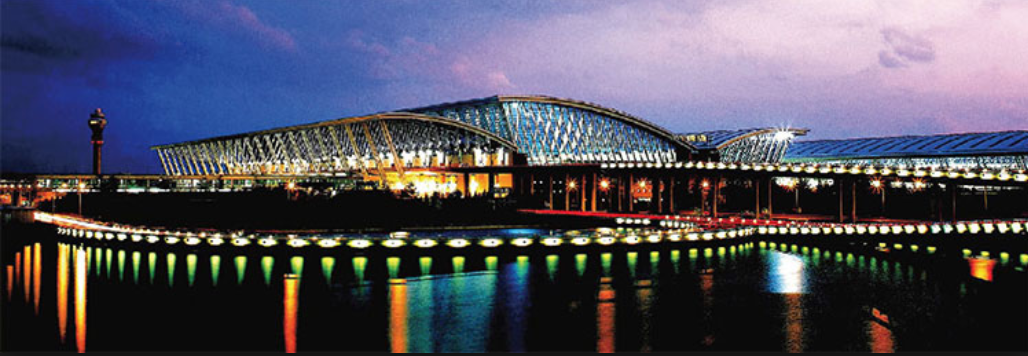
\includegraphics[width=0.8\textwidth]{SPIA.png}
    \caption{Shanghai Pudong International Airport \cite{Google_SPIA}}
    \label{fig:SPIA}
\end{figure}

As a huge rendezvous for many passengers, Pudong Airport has put forward a large number of measures to evacuate passengers, such as the famous maglev, underground, and shuttle buses. This operates quite well during daytime. However, during midnight period(23:00-02:00) when travellers get off from the red-eye flight, there's simply not enough transport capabilities to ensure passengers arrive at their destination in a short time. According to official statistics from Shanghai Traffic Management Bureau(STMB), around 10,000 passengers are stranded at the airport, waiting for a home-ride for a long duration.

Thanks to the overwhelming trend of the Internet, some novel transportation concepts have been put forward to meet the public's demand, such bus service and car-hailing. STMB intends to devise a new bus-booking platform, combining the benefits of both bus service and car-hailing. This new app hopes to achieve a better passenger experience.

\subsection{Our Work}

We named the bus booking platform BusHub.

In our paper, we focus on maximizing platform's marketing profits, promoting user satisfaction, and receiving orders as many as possible.Our model achieves a good balance among them. Destination Selection Model and Route Selection Model generates a reasonable route. Bus Dispatching Model gets a decent bus-departing schedule. 

In section \ref{sec:assu}, we state four basic assumptions. Section \ref{sec:Nome} is made up of the nomenclature used in the model statement. Section \ref{sec:stat} provides sufficient details about our proposed. Section \ref{sec:impl} implements our model with given and collected data. We conduct several targeting experiments and analyze our model in section\ref{sec:mode}. At last, we make our conclusions and devise an advertisement for our app in section \ref{sec:conc} and section \ref{sec:adve} respectively.

\section{Assumptions}\label{sec:assu}

Our model makes four assumptions as follows:

\begin{enumerate}
	\item In the phase of modeling, we consider each passenger as the same individual subject, and the taxi and bus GPS data on January 31st, 2007 statistically representative. We assume each passenger has the same standard for user satisfaction, namely satisfied if a bus is available while unsatisfied if not. Besides, we suppose there's little difference between the GPS data on the date we choose and others'.
	\item We use plane-coordinate system to replace spherical coordinates. Since Shanghai is not that big if seen from the globe, it is reasonable to assume like this.
	\item The GPS data typically reflects passengers' demands for buses' destinations. Since it's at deep night, there's few traffic jams. Besides, waiting time at the crossroads are randomly equal. 
	\item There is only one starting station, namely the Airport Station, and fifty terminal stations to choose from. All passengers need to go to the airport station to enjoy our bus-booking service. We don't take different airline landing site into account. 
	\item All the buses are the same, and seat 33 people. We simplify the bus to be used as the same standard bus, which has a fixed seat of thirty-three passengers averagely, based on our online research and calculation. Additionally, traffic accidents are ignored because it is rare, especially at night.
\end{enumerate}

\section{Nomenclature}\label{sec:Nome}
In this paper, we use the nomenclature in Table \ref{tab:Nomen} to describe our model. Other symbols that are used only once will be described later in the context.
\begin{table}
    \centering
    \caption{Nomenclature}
    \label{tab:Nomen}
    \begin{tabular}{c c}
\hline
    	Symbol & Definition\\
\hline
	$x$ & The longitude of each map point\\
	$y$ & The latitude of each map point\\
	$P(x,y)$ & The population density of each map point\\
	$T(x,y)$ & The taxi and bus GPS-recognized position density or traffic density\\
	$M(x,y)$ & The combined probability distribution of each map point\\
	$P_f$ & Acceptable risk ratio\\
	$Q(X_i;t)$ & Volumetric flow rate at time $t$ for dam $i$\\
\hline
    \end{tabular}
\end{table}

\section{Statement of our Model}\label{sec:stat}

In this section, we will discuss our model of predefined route cycles. This model has two major aspects. To begin with, we investigate population density and transportation density of Shanghai to select potential destinations. Then, we provides potential routes for buses, based on selected destinations. This model achieves a great balance between cost and user satisfaction. Chongmin Island is not taken in account, because it's barely unseen in transportation density, and longitude, along with latitude, is replaced by plane coordinates.

\subsection{Destination Selection Model}

\begin{figure}[h]
    \centering
    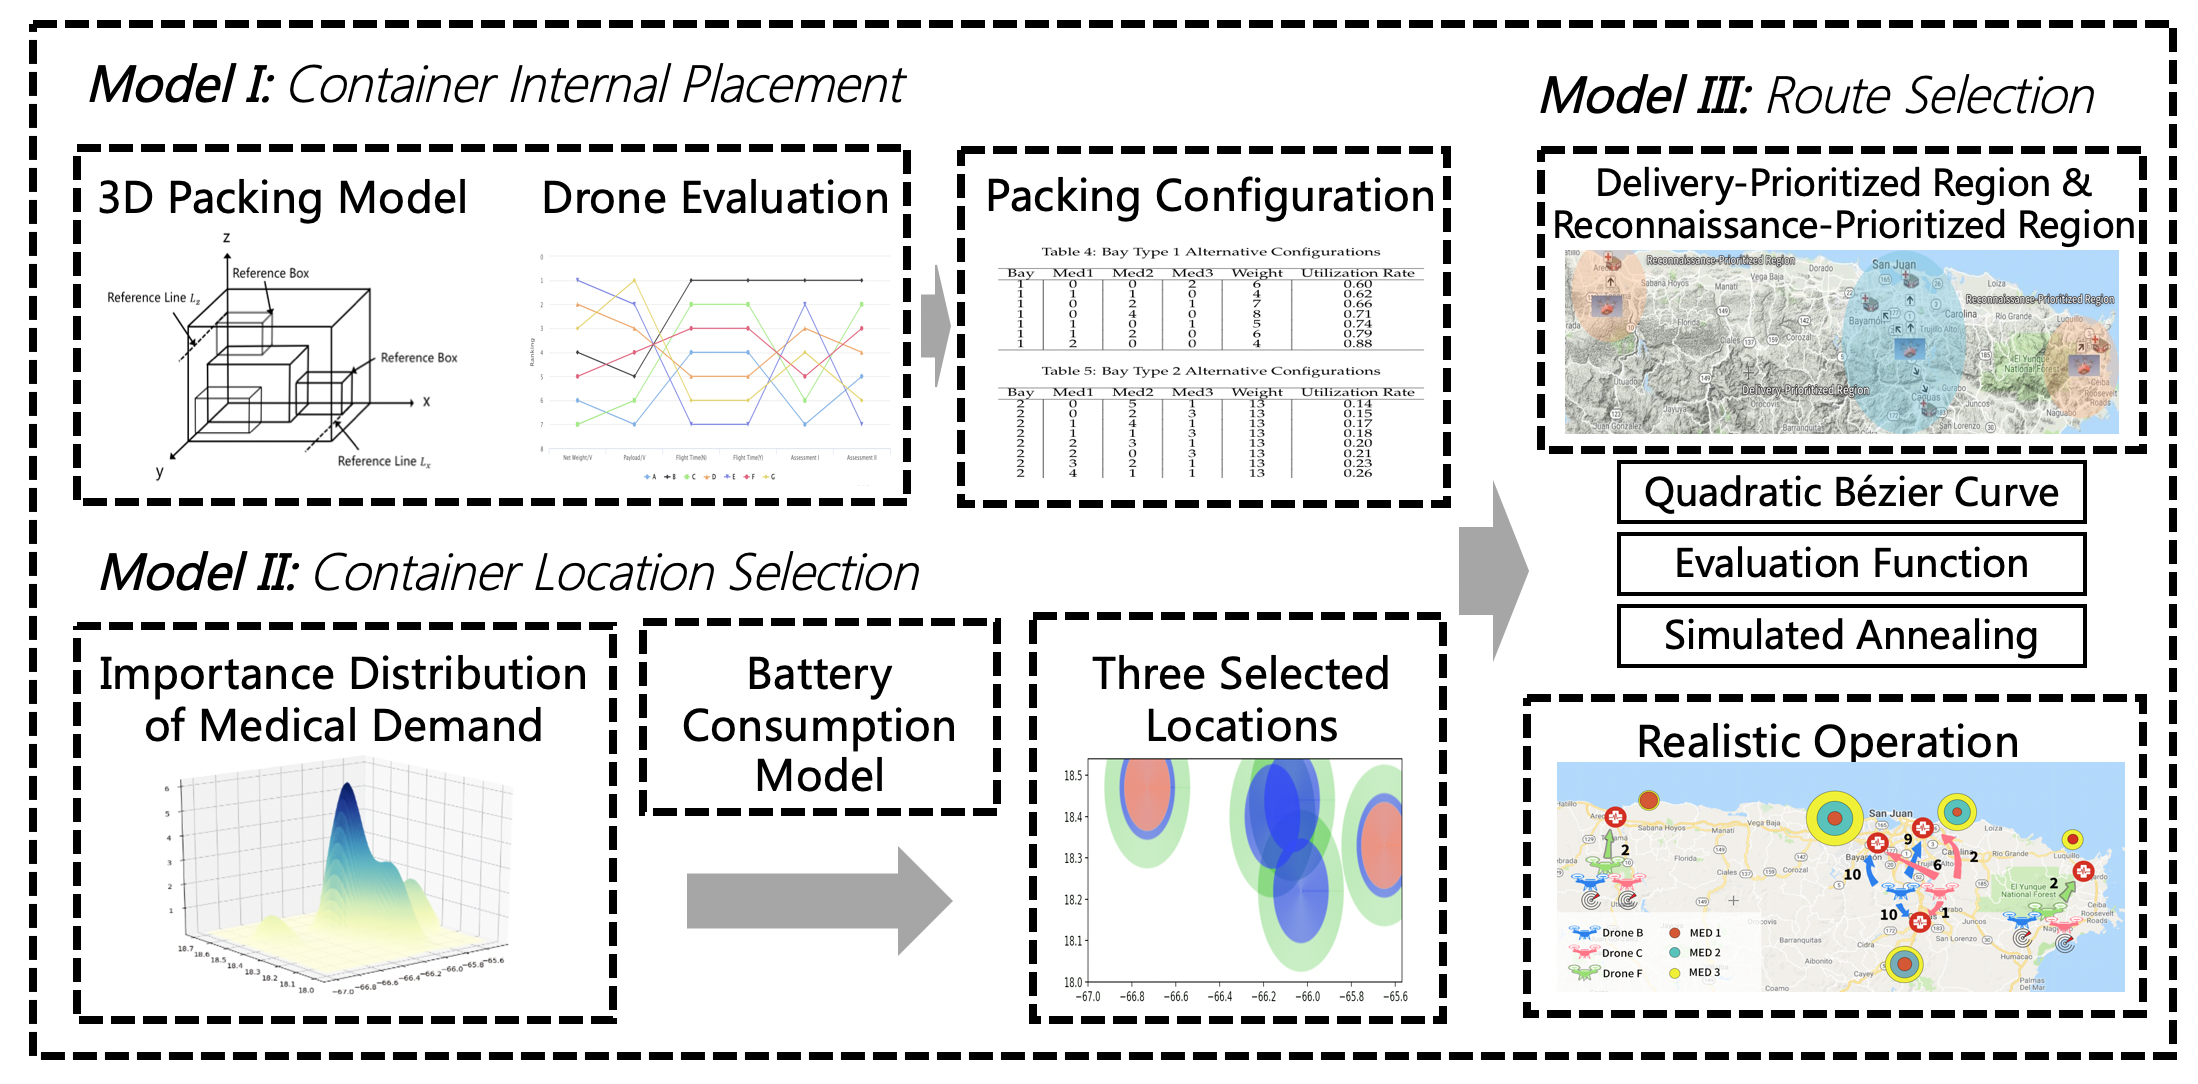
\includegraphics[width=0.8\textwidth]{figures/flowchart.png}
    \caption{Flow Chart of Destination \& Route Selection Model}
    \label{fig:flowchart}
\end{figure}

In our model, we need to select fifty hot destinations for passengers to choose from as their destination station. The population density function $P(x,y)$, and the traffic density $T(x,y)$ are taken into account to form a synthetical destinaiton selection function.

\subsubsection{Destination Selection Function}
In actual situations, for map points with higher population density rate or higher traffic density rate, we are more likely to select these points as our potential destination stations. More people in a certain area means more demands in the region, while more traffic density means people choose to go to these places at that time. 

We use the harmonic mean of $P(x,y)$ and $T(x,y)$ as our final destination selection function $M(x,y)$ to estimate potential destinations probability. This is because the harmonic mean reflects both influence factors evenly. Surely, there are some map points where the traffic density is much higher than population density, but we should take both factors into account, as both matter.

\begin{equation}\label{eq_product&sum}
    M(x,y) = \frac{P(x,y) \times T(x,y)}{P(x,y) + T(x,y)}
\end{equation}

For every map point $(x,y)$, the larger $M(x,y)$ is, the greater possibility for $(x,y)$ to be chosen as a destination. With this formula, we generate a chart on which we can preliminarily see the distribution of potential sites.

\subsubsection{Using Algorithms to Confirm Destinations}
We employ \emph{Metropolis-Hasting Algorithm(MHA)} to sample the function $M(x,y)$, and generate \textbf{potential destinations}. MHA is a Markov Chain Monte Carlo method, which can generate samples of a distribution function proportional to a given function, without normalizing it. Since $M(x,y)$ is a complicated function in two-dimensional space, it's impossible to integrate over the domain. But with MHA, we can still sample this function. Here we obtain a large number of points by MHA to explore where passengers are most likely to arrive at.

Afterwards, \emph{K-Means Clustering} is applied to get reasonable clusters, by which we finalize our selection of \textbf{fifty destination stations}. Additionally, if there are some bad points in them, we can also intervene into the generation of these destinations, but this accounts for only a small part.  In order to satisfy passengers' need as much as possible, we use K-Means to get \emph{k clusters} and set the stations at the heart of \emph{k clusters}. By this, we can \textbf{maximize} the area that buses cover and \textbf{minimize} the average distance between station and passengers' destination. For safety reasons, k is set a little larger than fifty to get rid of undermined bad points.

\subsection{Route Selection Model}
In this section, we introduce the cost function to select routes, and there are three elements influencing the cost function, \textbf{distance, population, and traffic conditions}. There are already fifty generated destinations , and we consider each as a key node. Possible route cycles only connect these nodes. 

\subsubsection{Integration}\label{sec:inte}
Distance(d), population(p), and traffic conditions(t) is mathematically stated as follows:
\begin{equation*}
    \begin{split}
        d &= |x_i-x_j| + |y_i-y_j|\\
        p &= P(x,y)\\
        t &= \int_{l}T(x,y)dl
    \end{split}
\end{equation*}

After researching, we normalize $d_e$, $t_e$ and $p_q$ by applying:
\begin{equation*}
    \hat{D}=\frac{D - min}{max - min} \qquad \& \qquad \hat{X}=\frac{X}{\sum X_i}\left(\text{X=$d_e$ or $p_q$}\right)
\end{equation*}

As we can see, $d_e$ is positively related, while $t_e$, and $p_q$ is negatively related to the cost function. This makes sense, since each bus has to be fueled per kilometre, and better traffic conditions as well as more seat occupancy rate contribute to larger number of turns and higher ticket sales.
The problem is now turned into an optimization problem, and \textbf{the cost function} is in the following presence.
\begin{equation}
\begin{aligned}	
    & \min\,\, Cost = \sum\limits_{Route\,\textbf{i}}(c_d \sum\limits_{e\in E_i} d_e + c_t \sum\limits_{e\in E_i} \frac{1}{t_e} + c_p \frac{1}{\sum\limits_{q\in Q_i} p_q})\\
    & s.t. \qquad
    \begin{cases}
    \bigcup\limits_{i}Q_i = Q, & |Q| = 50,\\
    \bigcup\limits_{i}E_i = E, & |E| = 50.
    \end{cases}
\end{aligned}
\end{equation}
where:
\begin{itemize}
    \item $e$, and $q$ are the corresponding elements of sets $E_i$ and $Q_i$;
    \item $E_i$ is the set of \textbf{edges} in \emph{route i};
    \item $Q_i$ is the set of points of destination stations we select;
    \item $d_e$ is the distance of each edge e, and $(x_i,y_i)$ \& $(x_j,y_j)$ are the endpoint of each edge;
    \item $t_e$ is the line integral of each edge;
    \item $p_q$ is the $P(x,y)$ of each destination.
\end{itemize}

Based on the Cost function, we successfully get 6 routes that best suits our model. There are six routes, because according to our analysis, if there are five or less routes, passengers diversified demands are not met properly; if there are more than six routes, different routes are quite similar to each other, which is obviously a waste of our existing transport capacity.

\subsubsection{Ranking model with AHP}

The \emph{Analytic Hierarchy Process(AHP)} is a structured technique for organizing and analyzing complex decisions, based on mathematics and psychology. Our goal is to rank three factors of the cost function and assign weights to each of them.

\begin{table}[h]
    \centering
    \caption{AHP production}
    \label{tab:AHP}
    \linespread{1.5}
    \begin{tabular}{c c}
\hline
    	Coefficient & Weight\\
\hline
	$c_d$ & 0.5403\\
	$c_t$ & 0.3478\\
	$c_p$ & 0.1119\\
\hline
    \end{tabular}
\end{table}

Table \ref{tab:AHP} shows the result of AHP. We then assign them to the model derived in Section \ref{sec:inte}:

\begin{equation}
\begin{aligned}	
    & \min\,\, Cost = \sum\limits_{Route\,\textbf{i}}(0.5403 \sum\limits_{e\in E_i} d_e + 0.3478 \sum\limits_{e\in E_i} \frac{1}{t_e} + 0.1119 \frac{1}{\sum\limits_{q\in Q_i} p_q})\\
    & s.t. \qquad
    \begin{cases}
    \bigcup\limits_{i}Q_i = Q, & |Q| = 50,\\
    \bigcup\limits_{i}E_i = E, & |E| = 50.
    \end{cases}
\end{aligned}
\end{equation}

\subsection{Bus Dispatching Model}

\begin{figure}[htbp]
    \centering
    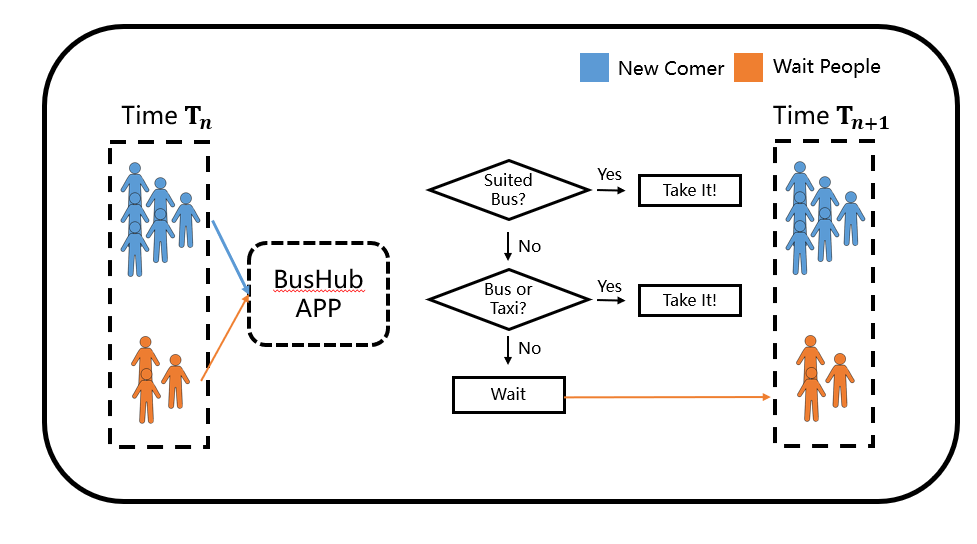
\includegraphics[height=8.5cm,width=16cm]{figures/APP.png}
    \caption{How BusHub works}
    \label{fig:BusHub}
\end{figure}

\subsubsection{Simulation of each passenger}

For each flight, we suppose the time people walk out of the airport is roughly in line with the normal distribution. This is reasonable, since the majority number of people walk out of the airport at the same time and only a few passengers come out early or late. Therefore, passengers-generated function is subject to normal distribution with multiple peaks.

For each passenger, we suppose that he uses our APP BusHub in the first place, as our service is cheap and timely. Within one minute, BusHub will respond whether there's a suitable bus for the user or not. As a result, he may choose other means to leave the airport, such as calling a taxi or stick to trying to book the next bus again. From the previous data, we assume the possibility of a passenger calling a taxi or riding on a shuttle bus is 7000/18000 and 1200/18000 respectively. If unfortunately, though, passengers failed to get on any of the vehicle mentioned above, they would have to wait for the platform to arrange another bus for them, as vividly shown in Picture \ref{fig:BusHub}.

For each bus, it will be back if it arrive at the final station in the route or there is no passenger on the bus after a while. (tkj)

\subsubsection{Greedy Algorithm}

\text{根据我们的cost函数和所得的路线,每个乘客的目的地在每条路线上是大致平均的。所以不会导致一条路线迟迟满不了一车的情况。再者,由于我们选的50个station所满足的条件,不会出现一个station下车人数远远小于其他station的情况。所以,我们的选的路线和station都是比较好的,不会出现特别极端的情况。由于各个路线的情况不会差距过大(price, distance, traffic),对于大人流的情况车是稀少的,我们采用贪心算法用来决定每辆车走哪个路线载哪些人是可行的。}

\text{关于定价,我们对每个station分别定价,采取分级定价策略。可以提高用户的满意度,降低部分乘客所需花费。这在app上是比较方便的。关于价格函数,它与距离和交通情况有关,与距离正相关,距离越大,价格越高,与交通情况负相关,交通越好,价格越低。为了平衡收益与用户满意度,我们设置价格函数是一个关于距离和交通的上凸函数。}











\section{Implementation}\label{sec:impl}
We tried to find some existing data set about the population density of Shanghai. but failed. However, we successfully find a colorfully-pointed graph, which indicates the population density. $P(x,y)$ is generated through the graph. With knowledge and techniques in digital image processing, we use the population density assigned to each color and color distribution, as well as noise reduction methods to get the two-dimension mathematical function $P(x,y)$. $T(x,y)$ is acquired through the given data set. Form the given data set, we assign a limited value to each existing map point. We take the longitude, latitude, speed, and status(occupied) into account, after which we apply convolution techniques to relevant values in order to form a two-dimension mathematical function $T(x,y)$. There are two charts below in Figure \ref{fig:two}, showing the two function's distribution.

\begin{figure}[htbp]
    \begin{minipage}{0.44\linewidth}
      \centerline{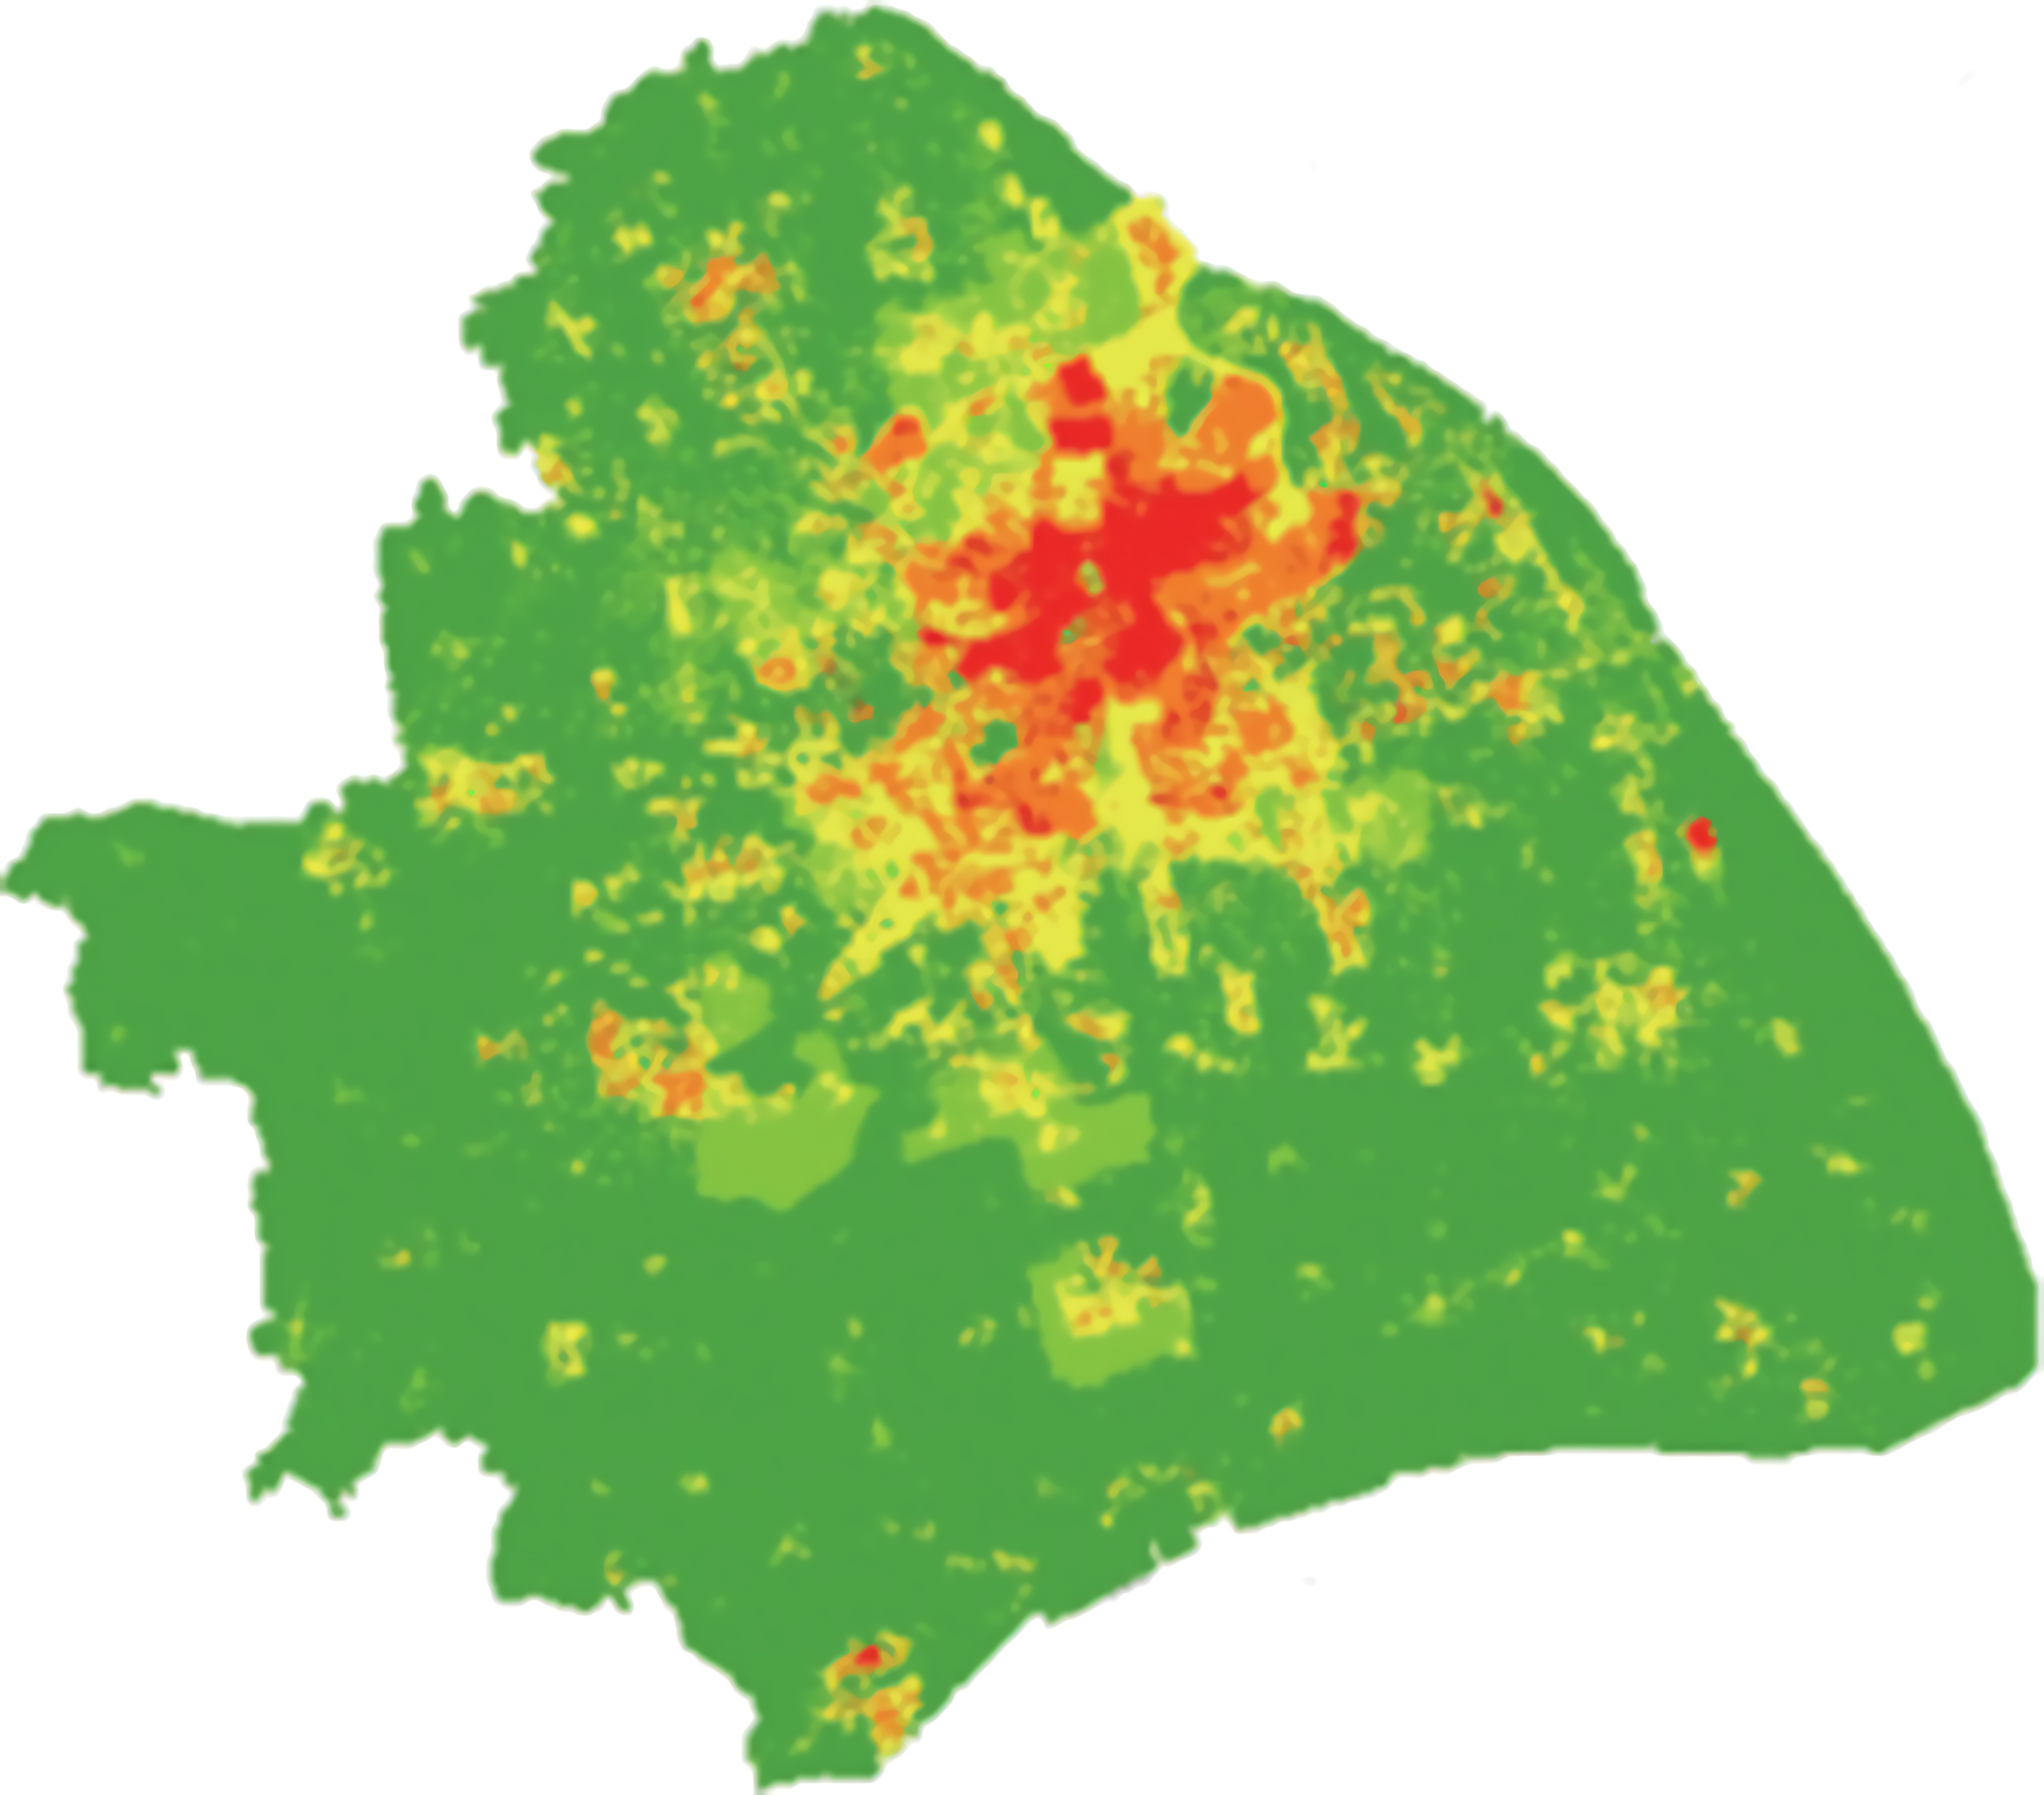
\includegraphics[height=5cm,width=7cm]{figures/Pd.jpg}}
      \caption*{(a) Population Density of Shanghai.}
    \end{minipage}
    \hspace{0.5in}
    \begin{minipage}{0.44\linewidth}
      \centerline{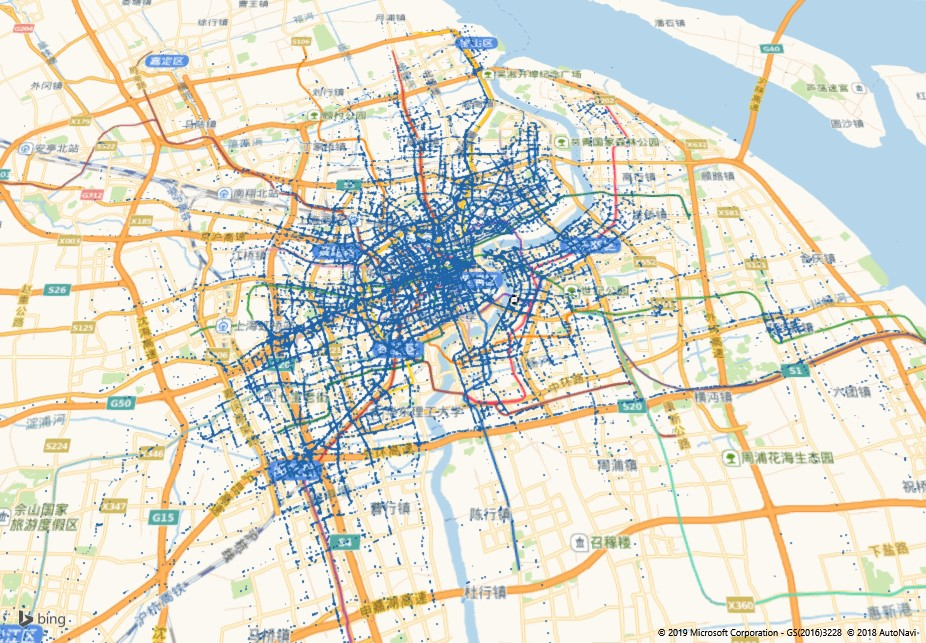
\includegraphics[height=5cm,width=7cm]{figures/Tran.png}}
      \caption*{(b) Traffic Density of Shanghai at midnight.}
    \end{minipage}
    \caption{Generation of fifty Destinations}
\end{figure}

In order to get smooth function images of $P(x,y)$ and $T(x,y)$, Gaussian Low Pass Filter (GLPF)~\cite{DigitalImageProcessing} is applied to our sampling. The two-dimension version function of the filter is

\begin{equation}
    \begin{split}
      H(u,v)     & =   e^{-D^2(u,v)/2\sigma^2}\\
                 & =   e^{-9D^2(u,v)/2R^2}
    \end{split}
\end{equation}

where:
\begin{itemize}
\item $D(u,v)$ is the distance from the center of the frequency rectangle;
\item $\sigma$ is a measure of the degree of central expansion, which is equal to $\left( \frac{R}{3} \right)$;
\item $R$ is the precision radius, which is equal to 600 metres.
\end{itemize}

Then, we acquire a reasonable distribution of $M(x,y)$. Its picture is shown in Figure\ref{fig:M(x,y)}:

\begin{figure}[htbp]
    \centering
    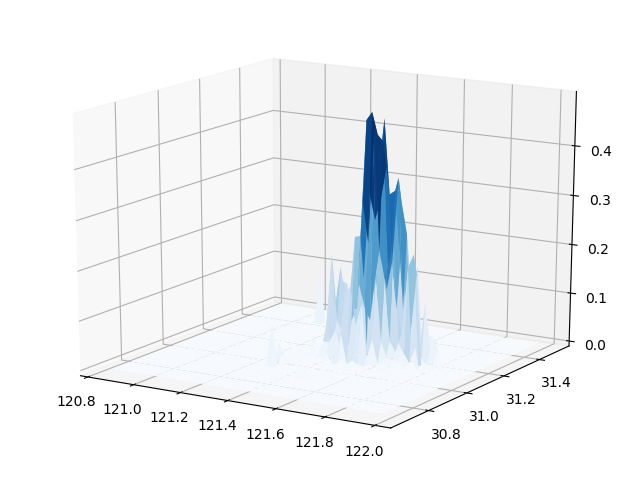
\includegraphics[height=5cm,width=7cm]{figures/M(x,y).png}
    \caption{Distribution of M(x,y)}
    \label{fig:M(x,y)}
\end{figure}

Afterwards, we use the Destination Selection Model and Route Selection Model to generate potential destinations, and finally integrate them into fifty destination stations. These two steps are depicted in Figure \ref{fig:twoII}.

\begin{figure}[htbp]
    \begin{minipage}{0.44\linewidth}
      \centerline{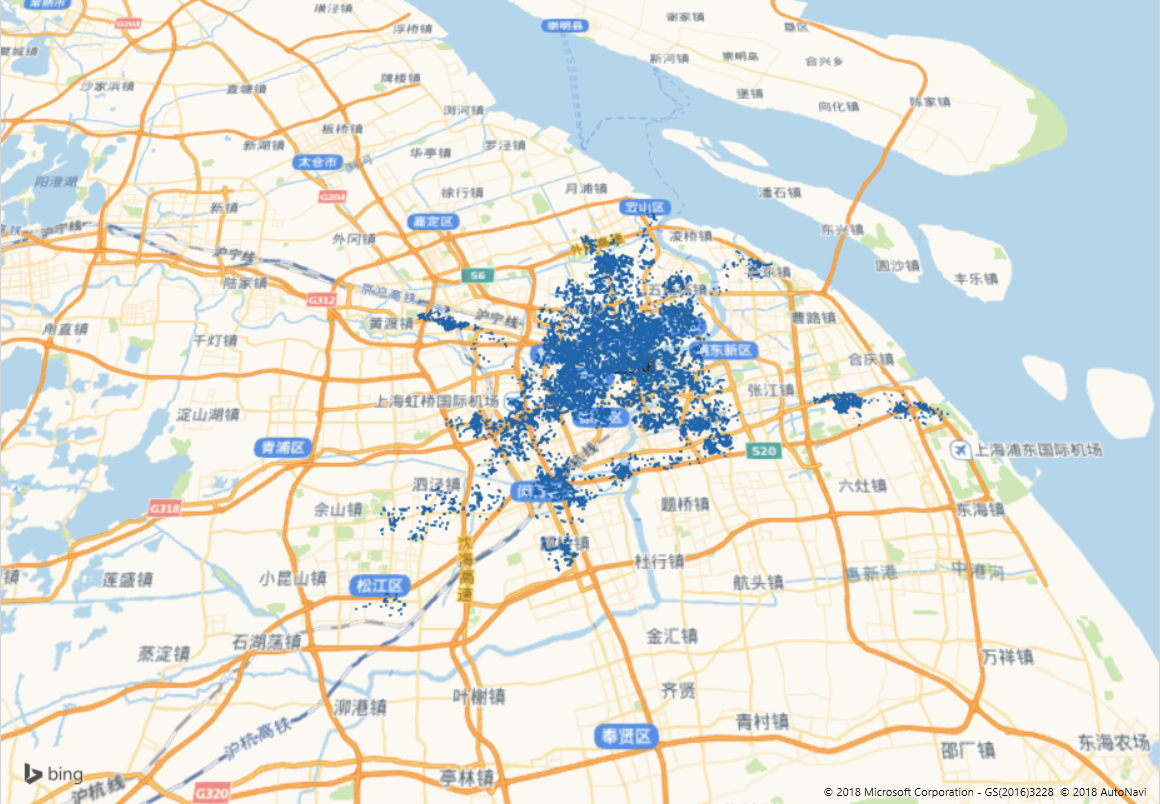
\includegraphics[height=5cm,width=7cm]{figures/PotentialDetinations.png}}
      \caption*{(a) Distribution of Potential Destinations.}
    \end{minipage}
    \hspace{0.5in}
    \begin{minipage}{0.44\linewidth}
      \centerline{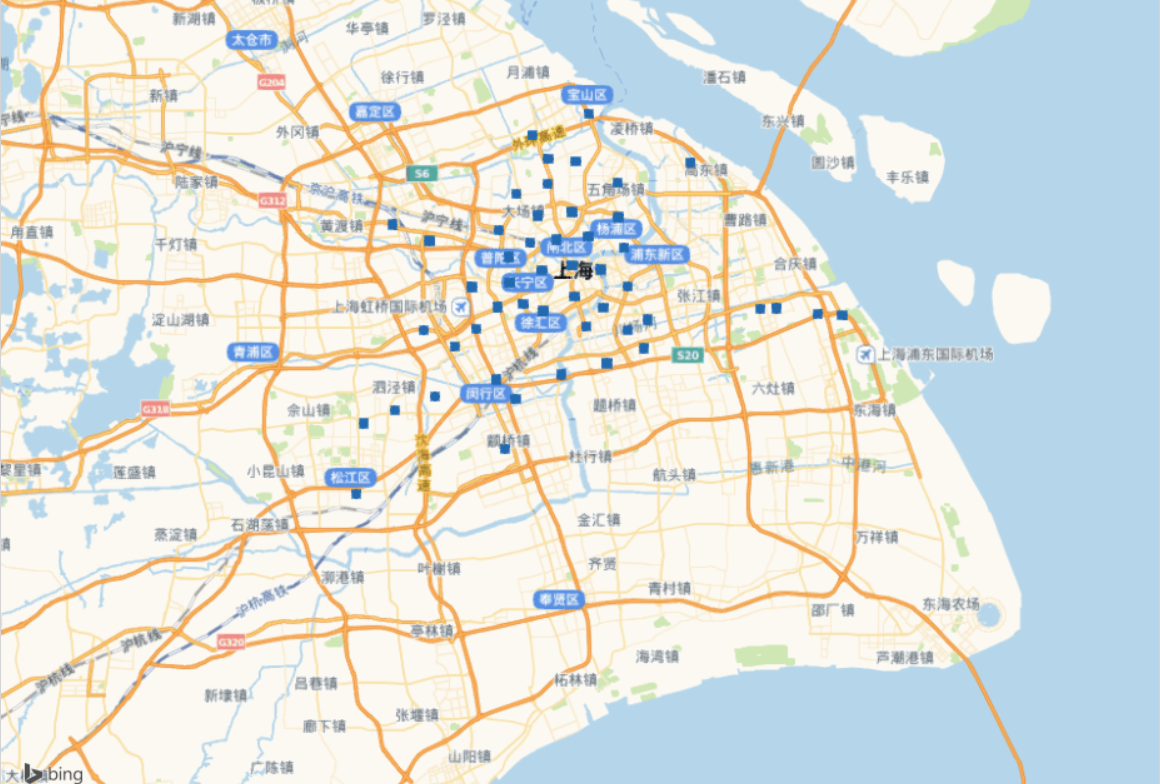
\includegraphics[height=5cm,width=7cm]{figures/fiftydestinations.png}}
      \caption*{(b) Distribution of fifty Destinations.}
    \end{minipage}
    \caption{Generation of fifty Destinations}
    \label{fig:twoII}
\end{figure}




We turn the destination address from the longitude-latitude form to detailed text address in Chinese. Thus, the APP can be more user-friendly. We extract a part of the total destinations shown in Figure\ref{fig:AIC}. All destinations are clearly set out in the appendix.

\begin{figure}[htbp]
    \centering
    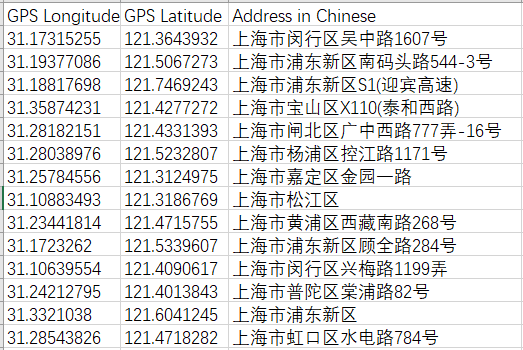
\includegraphics{figures/AddressinChinese.png}
    \caption{Part of the Destinations' Addresses in Chinese}
    \label{fig:AIC}
\end{figure}


Based on the three main models mentioned above, the bus-booking platform is integrated as a newly-released APP \text{BusHub} to meet customers' demands. BusHub receive orders, calculate backstage, and send feedbacks within one minute. In order to promote customer loyalty and user satisfaction, BusHub goes to great lengths to satisfy as many orders as possible. The following diagram shows how it works.


\section{Model Analysis}\label{sec:mode}
\subsection{Sensitivity Analysis}

\subsubsection{bus number}
\begin{figure}[htbp]
    \centering
    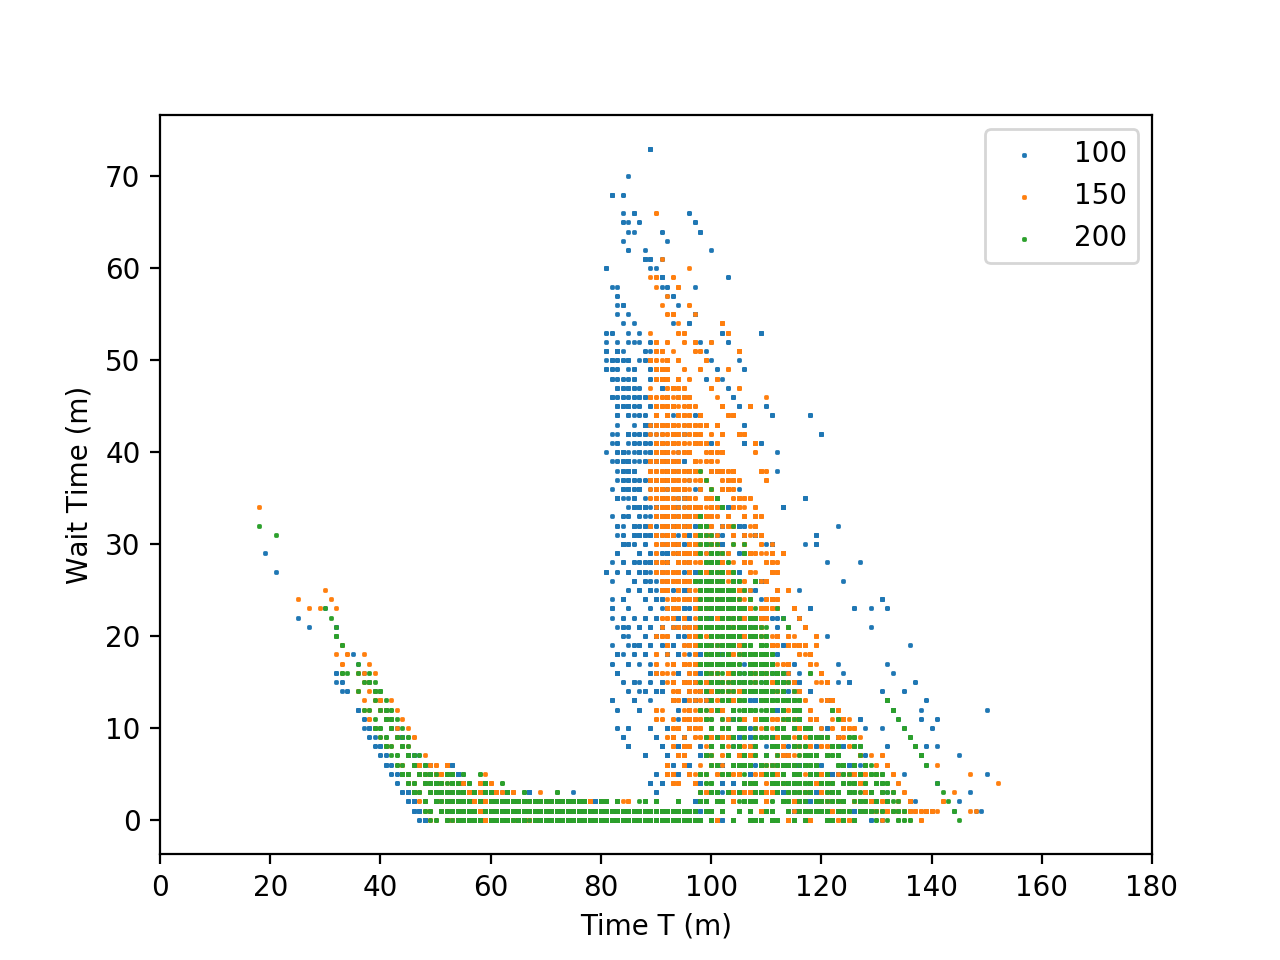
\includegraphics{figures/waittime.png}
    \caption{Wait time-Arrival time figure}
    \label{}
\end{figure}

describe and explain the figure. 
and 
bus number=100
taxi_and_bus= 8049
carry_how_many_people= 6864
average_living_time= 11.755973193473194
bus number=150
taxi_and_bus= 8220
carry_how_many_people= 9669
average_living_time= 10.971765435929258
bus number=200
taxi_and_bus= 8097
carry_how_many_people= 9834
average_living_time= 3.9335977221883263

\subsubsection{Routes Number}
For n < 6, less number of routes  cause that 

AHP, routes number, car number

\subsection{Strengths and Weaknesses}
\subsubsection{Strengths}
\begin{enumerate}
    \item We have reasonable and accurate sources of data, and our model is logically rigorous. During our brainstorm, we come up with many tough conditions, and revise the generated model to be more user-friendly.
    \item Our model is also interdisciplinary and practical. We use some classic knowledge and techniques in digital image processing. We
    conducted a lot simulations to test our model, and receive a good outcome.
    \item We use fancy visualization and clear diagram to state our model.
    \item We work hard to design the user interface of our app BusHub, and give our customer a nice access.
\end{enumerate}

\subsubsection{Weaknesses}
\begin{enumerate}
    \item Straight-line distance is used in our model. However, actual situation is more complex and tough. Spherical distance and Manhattan is more precise. 
    \item More real-life situations should be taken into account, such as real-time traffic conditions, and traffic density differences between day.
    \item Passengers' advice is important, too. Their opinion on route and destination selection also matters.
\end{enumerate}

\section{Conclusion}\label{sec:conc}
Our paper provides a detailed analysis of

\newpage\label{page}
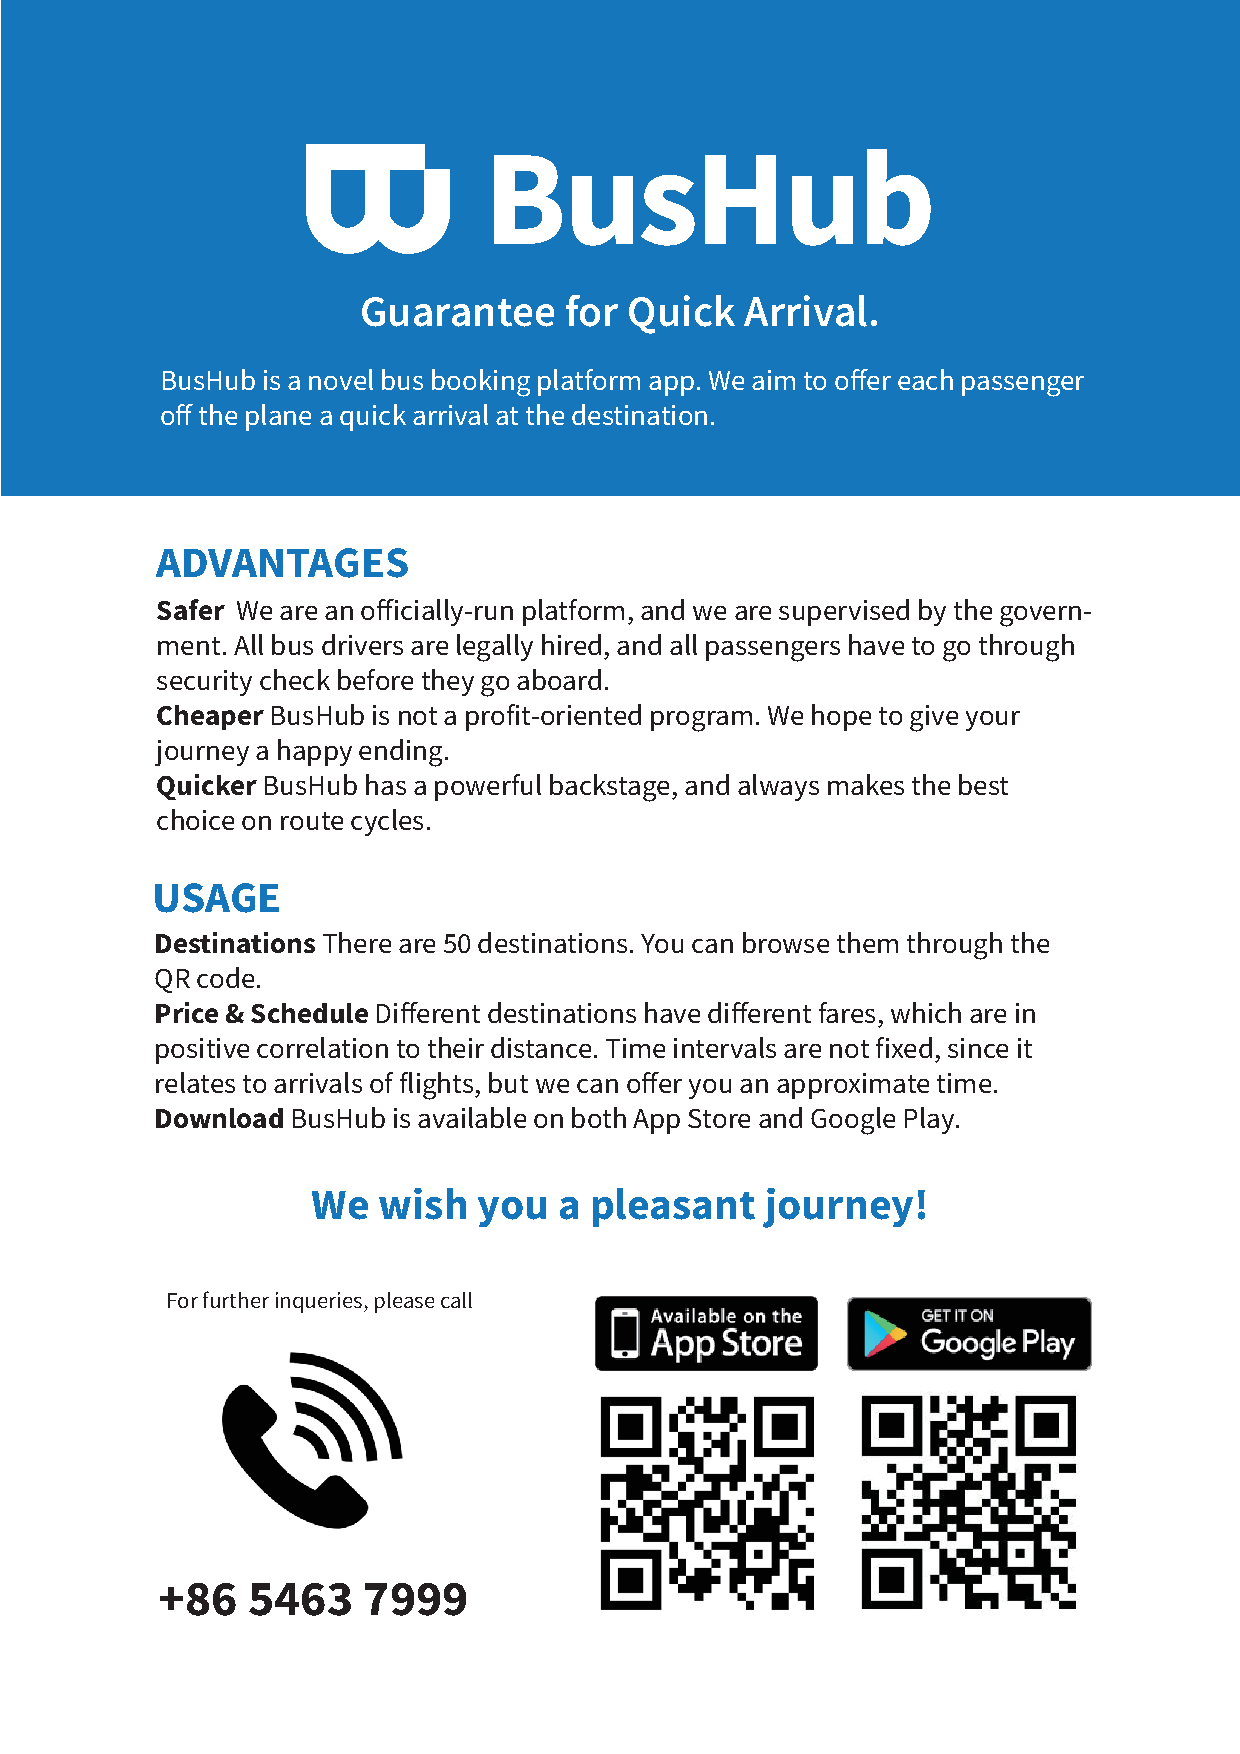
\includepdf[pages={1}]{123.pdf}

\section{Advertisement}\label{sec:adve}
Our advertisement is shown upward in Page\ref{page}.

\bibliographystyle{IEEEtran}
\bibliography{newrefs}

\newpage
\begin{appendices}
\section{Fifty Selected Destinations}
% Table generated by Excel2LaTeX from sheet 'Stations'
\begin{table}[htbp]
  \centering
  \caption{Longitude and Latitude of Fifty Destinations}
  \renewcommand\arraystretch{1.35}
    \begin{tabular}{|c|c|}
    \multicolumn{2}{c}{Fifty Destination Stations} \\
    \hline
    Longitude & Latitude \\
    \hline
    121.364393162531  & 31.173152552460  \\
    121.506727261692  & 31.193770863610  \\
    121.746924348685  & 31.188176982499  \\
    121.427727151510  & 31.358742313098  \\
    121.433139324850  & 31.281821514808  \\
    121.523280704171  & 31.280389760460  \\
    121.312497485300  & 31.257845558004  \\
    121.318676931596  & 31.108834932138  \\
    121.471575456181  & 31.234418142819  \\
    121.533960720319  & 31.172326196662  \\
    121.409061703513  & 31.106395542063  \\
    121.401384292276  & 31.242127947224  \\
    121.604124514158  & 31.332103796933  \\
    121.471828168427  & 31.285438256653  \\
    121.230262324458  & 31.015230791544  \\
    121.700675726468  & 31.193410339600  \\
    121.238600547066  & 31.083179839898  \\
    121.489783526947  & 31.262117133953  \\
    121.402093037180  & 31.218021052389  \\
    121.438025579592  & 31.229559793646  \\
    121.459520619477  & 31.129833350839  \\
    121.271084910573  & 31.273177521576  \\
    121.445246934034  & 31.336013691238  \\
    121.529393896826  & 31.251364350760  \\
    121.387172859152  & 31.124929047336  \\
    121.439640469256  & 31.191039080854  \\
    121.306396260030  & 31.172488372549  \\
    121.476011627950  & 31.333448666715  \\
    121.397037102902  & 31.058798512089  \\
    121.522513215793  & 31.313030242158  \\
    121.454646336302  & 31.258801946350  \\
    121.487640064119  & 31.176185161081  \\
    121.388412091579  & 31.194354995338  \\
    121.390018516950  & 31.267699508414  \\
    121.341503761017  & 31.156572158483  \\
    121.556704519879  & 31.182669427071  \\
    121.773870135207  & 31.186969896870  \\
    121.552350935580  & 31.154895396208  \\
    121.273777676284  & 31.096099848443  \\
    121.425089224955  & 31.256263202675  \\
    121.409972105050  & 31.302694807414  \\
    121.359945503646  & 31.213554954933  \\
    121.504103558526  & 31.230112052397  \\
    121.444298701623  & 31.312259258587  \\
    121.417223173704  & 31.197270242250  \\
    121.511163311648  & 31.140525418237  \\
    121.533558672333  & 31.213915495691  \\
    121.681836497288  & 31.192687075444  \\
    121.474509588538  & 31.204650653065  \\
    121.491086492494  & 31.378981942682  \\
    \hline
    \end{tabular}%
  \label{tab:addlabel}%
\end{table}%

\newpage
\section{Implemented Algorithms and Codes}
\subsection{Metropolis Hastings \& Simulated Annealing Algorithm}
\lstinputlisting[language=python]{mtr.py}

\subsection{Population Density Estimate}
\lstinputlisting[language=python]{pop.py}

\subsection{Transportation Density Estimate}
\lstinputlisting[language=python]{traf.py}

\subsection{Destination Stations Selection}
\lstinputlisting[language=python]{stt.py}

\subsection{Route Selection}
\lstinputlisting[language=python]{rt.py}

\subsection{Simulation of each passenger}
\lstinputlisting[language=python]{simulation.py}
\end{appendices}
\end{document}


